\documentclass[aspectratio=169]{beamer}

\usepackage[T1]{fontenc}
\usepackage[utf8]{inputenc}
\usepackage{graphicx}
\usepackage{booktabs}
\usepackage{xcolor}
\usepackage{tikz}

\graphicspath{{../models/}}

% ---------------------------------------------------------------------------
% Gruvbox Light palette (https://github.com/morhetz/gruvbox). Light mode uses
% gruvbox's "neutral" (darker/muted) accent set, not the bright set used on
% dark backgrounds -- the bright colors don't have enough contrast on cream.
% ---------------------------------------------------------------------------
\definecolor{bglight}{HTML}{FBF1C7}  % bg0
\definecolor{bgraised}{HTML}{EBDBB2} % bg1
\definecolor{hairline}{HTML}{BDAE93} % bg3
\definecolor{txt}{HTML}{3C3836}      % fg1
\definecolor{txtdim}{HTML}{665C54}   % fg3
\definecolor{txtfaint}{HTML}{928374} % gray
\definecolor{amber}{HTML}{AF3A03}    % neutral orange
\definecolor{tealc}{HTML}{427B58}    % neutral aqua
\definecolor{slatec}{HTML}{7C6F64}   % fg4

\setbeamercolor{background canvas}{bg=bglight}
\setbeamercolor{normal text}{fg=txt}
\setbeamercolor{title}{fg=amber}
\setbeamercolor{subtitle}{fg=txtdim}
\setbeamercolor{author}{fg=txtdim}
\setbeamercolor{institute}{fg=txtdim}
\setbeamercolor{date}{fg=txtdim}
\setbeamercolor{frametitle}{fg=amber,bg=bglight}
\setbeamercolor{framesubtitle}{fg=txtfaint}
\setbeamercolor{structure}{fg=tealc}
\setbeamercolor{itemize item}{fg=tealc}
\setbeamercolor{itemize subitem}{fg=slatec}
\setbeamercolor{enumerate item}{fg=tealc}
\setbeamercolor{block title}{fg=amber,bg=bgraised}
\setbeamercolor{block body}{fg=txtdim,bg=bgraised}
\setbeamercolor{footlinecolor}{fg=txtfaint,bg=bglight}
\setbeamercolor{alerted text}{fg=amber}

\setbeamertemplate{navigation symbols}{}
\setbeamertemplate{itemize items}[triangle]
\setbeamerfont{frametitle}{series=\bfseries,size=\Large}
\setbeamerfont{title}{series=\bfseries,size=\huge}
\setbeamerfont{framesubtitle}{series=\mdseries,size=\scriptsize}

\setbeamertemplate{frametitle}{
  \vspace{0.3em}
  {\usebeamerfont{frametitle}\usebeamercolor[fg]{frametitle}\insertframetitle}\\[-0.1em]
  {\usebeamerfont{framesubtitle}\usebeamercolor[fg]{framesubtitle}\MakeUppercase{\insertframesubtitle}}
  \vspace{0.2em}
  \hrule height 0.4pt \color{hairline}
  \vspace{0.6em}
}

\setbeamertemplate{footline}{
  \leavevmode
  \hbox{%
    \begin{beamercolorbox}[wd=.5\paperwidth,ht=2.6ex,dp=1.2ex,left,leftskip=1em]{footlinecolor}
      \tiny\color{txtfaint} FLYROTOR \textperiodcentered\ AI-KF ON CRAZYFLIE
    \end{beamercolorbox}%
    \begin{beamercolorbox}[wd=.5\paperwidth,ht=2.6ex,dp=1.2ex,right,rightskip=1em]{footlinecolor}
      \tiny\color{txtfaint} \insertframenumber\,/\,\inserttotalframenumber
    \end{beamercolorbox}%
  }
}

\newcommand{\code}[1]{\textcolor{tealc}{\texttt{#1}}}
\newcommand{\stat}[1]{\textcolor{amber}{\textbf{#1}}}

\title{AI-KF on Crazyflie}
\subtitle{Estimating altitude without a height sensor}
\author{Toha \and Melanie \and Jaden}
\institute{BRAID 2026 Claude-o-thon}
\date{}

\begin{document}

% ---------------------------------------------------------------------------
\begin{frame}[plain]
  \begin{center}
    \vspace{0.2em}
    {\setlength{\fboxsep}{5pt}\setlength{\fboxrule}{0.6pt}\color{hairline}%
     \fbox{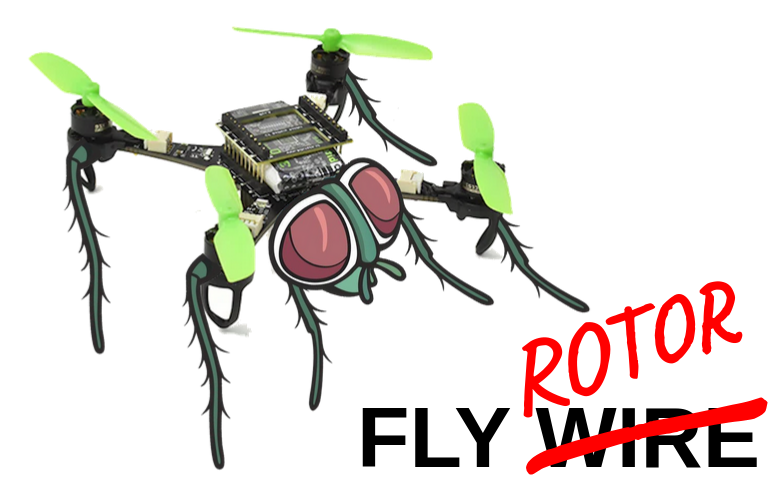
\includegraphics[width=6.4cm]{team_logo.png}}}\\[1.1em]
    {\usebeamerfont{title}\usebeamercolor[fg]{title}\inserttitle}\\[0.15em]
    {\usebeamerfont{subtitle}\usebeamercolor[fg]{subtitle}\insertsubtitle}\\[1.6em]
    {\usebeamercolor[fg]{author}\insertauthor}\\[0.7em]
    {\usebeamercolor[fg]{institute}\scriptsize\insertinstitute}
  \end{center}
\end{frame}

% ---------------------------------------------------------------------------
\begin{frame}{Background}
  \begin{itemize}
    \item The \textbf{AI-Kalman Filter} (Cellini et al.\ 2025) performs better than
      a standard Kalman filter for estimation in unobservable times.
    \vspace{0.6em}
    \item The \textbf{Crazyflie} is a small drone with the same sensors used in the 
          AI-KF paper. 
    \vspace{0.6em}
    \item This is a good opportunity to test the AI-KF on a real platform!
  \end{itemize}
\end{frame}

% ---------------------------------------------------------------------------
\begin{frame}{Project Goals}
  \begin{enumerate}
    \setlength{\itemsep}{1.1em}
    \item \textbf{Estimate on a collected trajectory} --- run the AI-KF estimator on
      real, already-logged flight data and validate it against the withheld ToF
      reading.
    \item \textbf{Real-time altitude estimation} --- run the same estimator live on the Crazyflie
    \item \textbf{Feed the control strategy} --- use the live estimate to actually
      inform how the drone is controlled, not just observe it.
      \hfill \textcolor{tealc}{\scriptsize\textsc{[stretch goal]}}
  \end{enumerate}
\end{frame}

% ---------------------------------------------------------------------------
\begin{frame}{146 real flights, seven motifs}
  \scriptsize
  \setlength{\tabcolsep}{4pt}
  \begin{table}
    \begin{tabular}{@{}l r p{6.2cm}@{}}
      \toprule
      \textbf{Motif} & \textbf{Reps} & \textbf{Why we flew it} \\
      \midrule
      \code{accel\_decel\_pulse} & \stat{96} & The key motif --- horizontal speed-up/slow-down is the only case the paper predicts makes altitude observable from flow + accel. \\[0.15em]
      \code{sum\_of\_sines} & \stat{16} & Continuous random-frequency acceleration, for frequency coverage beyond single pulses. \\[0.15em]
      \code{vertical\_bob} & \stat{8} & Negative control --- vertical-only motion, predicted near-zero observability. \\[0.15em]
      \code{offset\_turn} & \stat{8} & Coordinated yaw + forward turn, to decouple heading from velocity direction. \\[0.15em]
      \code{zigzag} & \stat{6} & Task-representative coverage pattern flown at near-deployment speed. \\[0.15em]
      \code{mixed\_free} & \stat{6} & Curated concatenation of motifs, closer to unstructured real flight. \\[0.15em]
      \code{hover} & \stat{6} & Baseline, low-observability control condition. \\
      \bottomrule
    \end{tabular}
  \end{table}
  \vspace{0.15em}
  \footnotesize
  \textcolor{txtfaint}{\texttt{146 reps total, across \textasciitilde 15 flights \textperiodcentered\ data\_collection/trajectories.py}}
\end{frame}

% ---------------------------------------------------------------------------
\begin{frame}{Trained directly on the real flights}{ANN training}
  \begin{columns}[T,onlytextwidth]
    \column{0.5\textwidth}
      \centering
      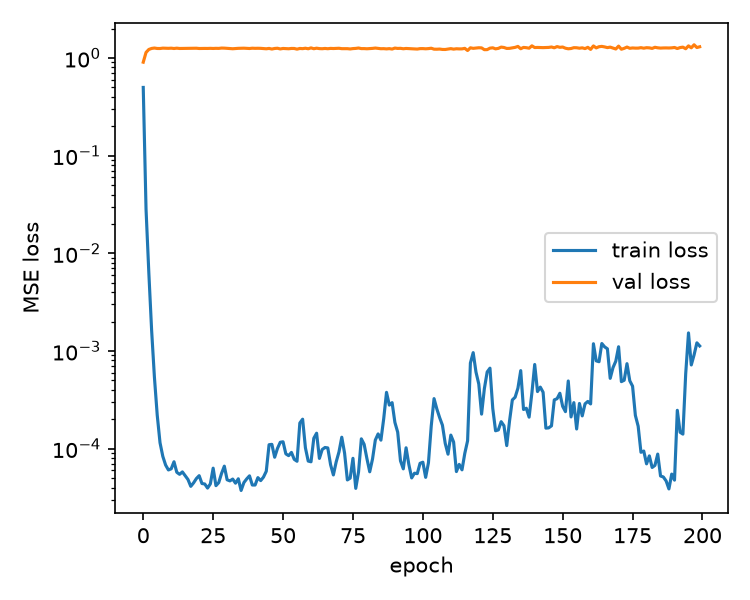
\includegraphics[height=3.55cm]{training_curve.png}\\
      \vspace{0.15em}\tiny\textcolor{txtfaint}{TRAINING CURVE}
    \column{0.5\textwidth}
      \centering
      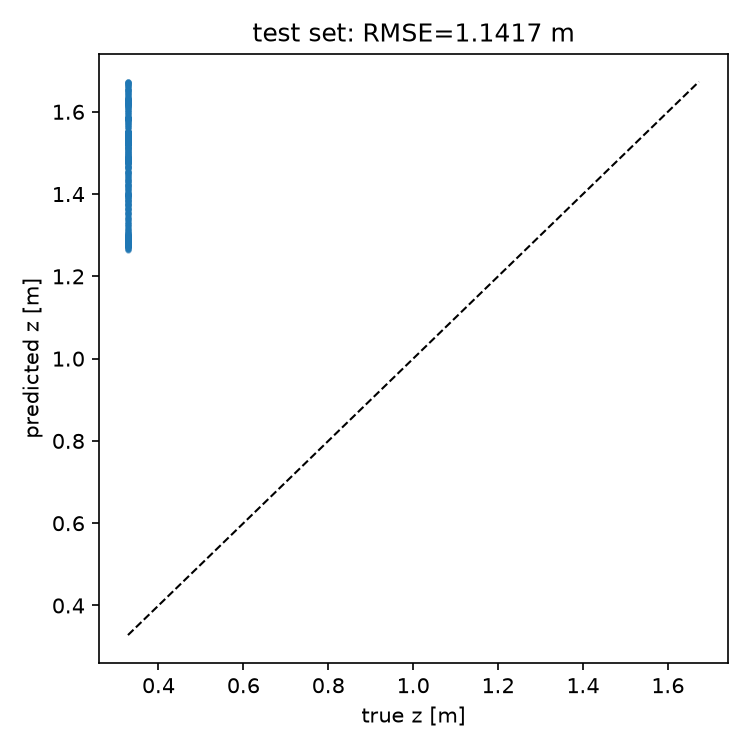
\includegraphics[height=3.55cm]{test_predictions.png}\\
      \vspace{0.15em}\tiny\textcolor{txtfaint}{TEST PREDICTIONS}
  \end{columns}
  \vspace{0.1em}
  \footnotesize
  A 3$\times$64 feed-forward net reads a sliding 2-second window (197 steps) of flow +
  accel and outputs altitude: \stat{109} training reps, \stat{30} held-out test reps,
  test \stat{RMSE = 2.53 cm}.
  \begin{block}{Caveat}
    \scriptsize
    Encouraging, but not conclusive: nearly every flight targeted the \textbf{same
    nominal 0.4~m} altitude, so this mostly shows the estimator tracking small
    in-flight height jitter, not large deliberate height changes. More height
    variation in training data is next.
  \end{block}
\end{frame}

% ---------------------------------------------------------------------------
\begin{frame}{Live estimation demo --- coming next}{Estimation}
  \centering
  \vspace{0.5em}
  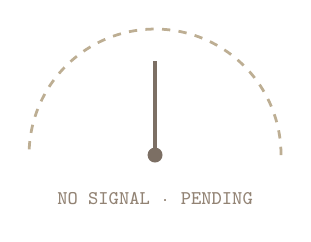
\begin{tikzpicture}
    \draw[hairline, dashed, line width=1pt] (0,0) arc[start angle=0, end angle=180, radius=1.6];
    \filldraw[slatec] (-1.6,0) circle (2.5pt);
    \draw[slatec, line width=1.5pt] (-1.6,0) -- (-1.6,1.2);
    \node[txtfaint, font=\scriptsize\ttfamily] at (-1.6,-0.55) {NO SIGNAL \textperiodcentered\ PENDING};
  \end{tikzpicture}
  \vspace{0.8em}

  \small
  \begin{minipage}{0.85\textwidth}
    \centering
    We don't have a live result to show yet. Once the tuned estimator is wired into
    the real-time fusion loop, this slide becomes a side-by-side of the AI-KF's fused
    altitude against the withheld ToF ground truth.
  \end{minipage}
\end{frame}

% ---------------------------------------------------------------------------
\begin{frame}{Three directions from here}{Future work}
  \begin{itemize}
    \setlength{\itemsep}{1.2em}
    \item \textbf{Broaden the observability analysis} --- we only recreated the
      sensor set from Ben's preprint. Worth running the same analysis on other
      sensors and states we haven't tried yet.
    \item \textbf{Scrutinize the drone model} --- check whether our model is actually
      accurate, or can be improved, and tune the Kalman filter's \textbf{Q} and
      \textbf{R} matrices instead of leaving them as placeholders.
    \item \textbf{Improve training} --- more height variation and more data,
      particularly to get past the ``single nominal altitude'' limitation in
      today's results.
  \end{itemize}
\end{frame}

\end{document}
